\documentclass[a4paper,12pt]{article}
\usepackage[french]{babel} 
\usepackage[T1]{fontenc}
%\usepackage[ansinew]{inputenc}
\usepackage[utf8]{inputenc}
\usepackage[top=3cm, bottom=3cm, left=2.3cm,right=2cm]{geometry}
\usepackage{graphicx}
\usepackage{color}
\usepackage{listings}
%\usepackage{marvosym}
%\usepackage{yfonts}
\usepackage[normalem]{ulem}
\usepackage{verbatim}
\usepackage{listings}
\usepackage{float}
%\renewcommand{\thesection}{\arabic{section}}
\usepackage{array} % pour les tableaux
\usepackage{amsmath} % pour les équations
\usepackage{float}
\usepackage{hyperref}	% crée des liens dans le pdf
\hypersetup{					% colorise les liens du pdf
	colorlinks=true,
	urlcolor=black
	citecolor=black,
	linkcolor=black,
	urlcolor=blue
}

% listes
\usepackage{enumitem}
\frenchbsetup{StandardLists=true} 
\renewcommand\labelitemi{$\bullet$}
\renewcommand\labelitemii{$\circ$}

\usepackage{url}			% change la police des url (utilisation : \url{http://asdf.ch})
\definecolor{dkgreen}{rgb}{0,0.6,0}
\definecolor{gray}{rgb}{0.5,0.5,0.5}
\definecolor{mauve}{rgb}{0.58,0.01,0.82}
%[babel=true]
\usepackage{csquotes}
\lstset{ %
	language=C,                % the language of the code
	basicstyle=\footnotesize,           % the size of the fonts that are used for the code
	numbers=left,                   % where to put the line-numbers
	numberstyle=\tiny\color{gray},  % the style that is used for the line-numbers
	stepnumber=1,                   % the step between two line-numbers. If it's 1, each line 
	% will be numbered
	numbersep=5pt,                  % how far the line-numbers are from the code
	backgroundcolor=\color{white},      % choose the background color. You must add \usepackage{color}
	showspaces=false,               % show spaces adding particular underscores
	showstringspaces=false,         % underline spaces within strings
	showtabs=false,                 % show tabs within strings adding particular underscores
	frame=single,                   % adds a frame around the code
	rulecolor=\color{black},        % if not set, the frame-color may be changed on line-breaks within not-black text (e.g. commens (green here))
	tabsize=2,                      % sets default tabsize to 2 spaces
	captionpos=b,                   % sets the caption-position to bottom
	breaklines=true,                % sets automatic line breaking
	breakatwhitespace=false,        % sets if automatic breaks should only happen at whitespace
	title=\lstname,                   % show the filename of files included with \lstinputlisting;
	% also try caption instead of title
	keywordstyle=\color{blue},          % keyword style
	commentstyle=\color{dkgreen},       % comment style
	stringstyle=\color{mauve},         % string literal style
	escapeinside={\%*}{*)},            % if you want to add a comment within your code
	morekeywords={*,...}               % if you want to add more keywords to the set
}

%Table of content with dot
\usepackage{etoolbox}
\makeatletter
\patchcmd{\l@section}
{\hfil}
{\leaders\hbox{\normalfont$\m@th\mkern \@dotsep mu\hbox{.}\mkern \@dotsep mu$}\hfill}
{}{}
\makeatother

%no indentation
\setlength{\parindent}{0cm}

%en-tête
\usepackage{fancyhdr}
\lhead{SEEE}
\chead{}
\rhead{\today}
\pagestyle{fancy}

% Title Page
\title{\Huge{\textsc{Internet of things}} \\ 
	\Huge{\textbf{Agricultural monitoring system}} \\
	\huge{Master HES-SO}}
\author{Émilie \textsc{Gsponer}, Grégory \textsc{Emery} }
\date{\today \\
	version 1.0}
%-------------------------début du document-------------------------------------
\begin{document}

\maketitle % page de garde
\newpage
\tableofcontents % table des matières
\newpage
\section{Introduction}
Le projet choisi est celui du système de monitoring pour l'agriculture. Son but est de collecter des données de plusieurs capteurs répartis dans un champ et de les transmettre à l'agriculteur peu importe où il se trouve sur la parcelle.\\\\
Dans le cadre de ce projet nous allons utiliser deux capteurs SensorTag qui communiquent en Bluetooth Low Energy (BLE) pour collecter des informations sur l'humidité, la température et la luminosité. Les données sont ensuite transmises à un contrôleur via BLE qui va analyser les informations et générer une alerte si les champs ont besoin d'être irrigués. Toutes les données collectées ainsi que l'alerte sont transmises au travers d'un réseau LoRaWAN.\\\\
Optionnelement nous pouvons implémenter une petite application permettant de voir les données et alarmes collectées par le réseau.\\\\
L'image ci-dessous représente notre système.
\begin{figure}[H]
	\begin{center}
		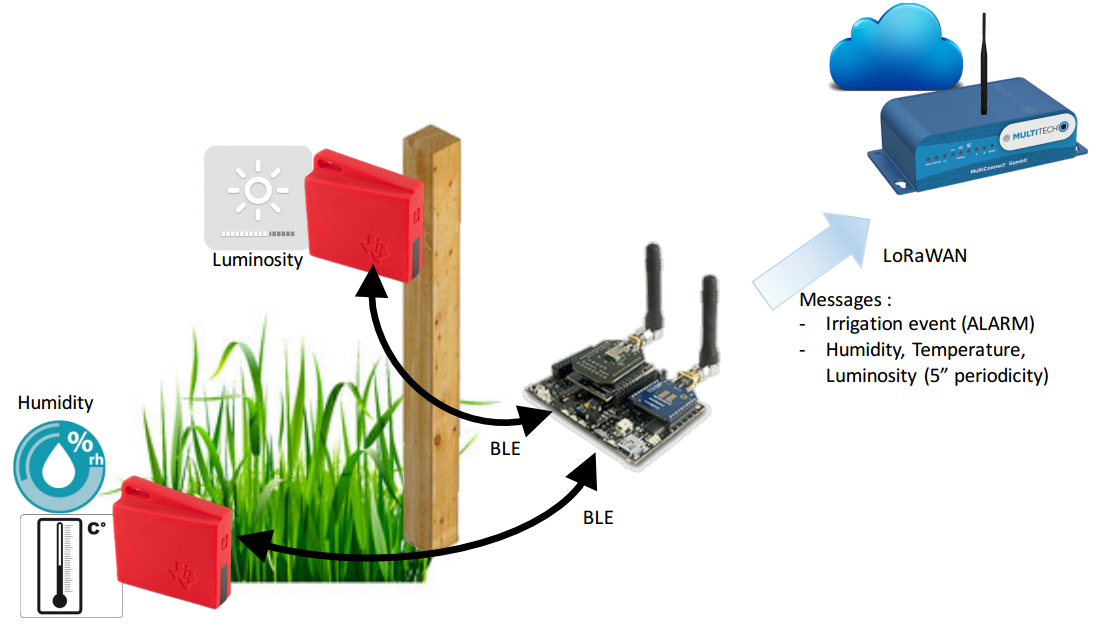
\includegraphics[width=17cm]{img/intro.png}
		\caption{Représentation du système}
		\label{intro}
	\end{center}
\end{figure}
\newpage
\section{Communication Bluetooth}
\subsection{Matériel à disposition}
Pour ce projet, nous avons pu avoir deux boîtes complètes à disposition. Voici quelques caractéristiques qui sont propres à ce matériel et utilisées dans ce projet.
\begin{itemize}
	\item SensorTag 1:
	\begin{itemize}
		\item Numéro du capteur: 9
		\item Mac adresse: b0:b4:48:c9:b3:85
		\item Données collectées: Luminosité 
	\end{itemize}
	\item SensorTag 2:
	\begin{itemize}
		\item Numéro du capteur: 16
		\item Mac adresse: b0:b4:48:c9:ba:01
		\item Données collectées: Température, Humidité 
	\end{itemize}
	\item Carte Bluetooth du Waspmote:
	\begin{itemize}
		\item Numéro du socket: 1
	\end{itemize}
\end{itemize}
\newpage
\section{Conclusion}

\end{document}


